\begin{qunlist}


\q{$\bigstar\bigstar$}{Minimal Positive Valued Function}

Consider a strictly decreasing function $f :
\mathbb{N} \rightarrow \mathbb{Z}$, such that $f(i) > f(i + 1)$ for all $i \in \mathbb{N}$. Assuming we can evaluate $f$ at any number in constant time, we want to find $n = \min\{i \in \mathbb{N}:f(i) < 0\}$. Design a $O(\log n)$ algorithm to compute $n$.

\textit{(Please turn in a four part solution to this problem.)}



\pagebreak

\q{$\bigstar\bigstar$}{Graph Basics}

For parts (a) and (b), refer to the figure below. For parts (c) through (f), please prove only for simple graphs; that is, graphs that do not have any parallel edges or self-loops.

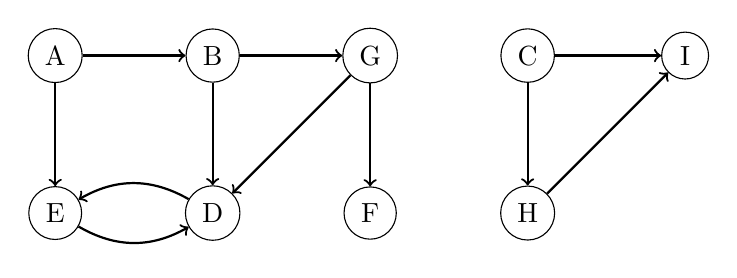
\begin{tikzpicture}
[ar/.style={->,thick},no/.style={draw,circle}]
\node [no] at (0cm,4cm) (A) {A};
\node [no] at (2cm,4cm) (B) {B};
\node [no] at (6cm,4cm) (C) {C};
\node [no] at (2cm,2cm) (D) {D};
\node [no] at (0cm,2cm) (E) {E};
\node [no] at (4cm,2cm) (F) {F};
\node [no] at (4cm,4cm) (G) {G};
\node [no] at (6cm,2cm) (H) {H};
\node [no] at (8cm,4cm) (I) {I};

\draw [ar] (A) -- (B);
\draw [ar] (A) -- (E);
\draw [ar] (B) -- (G);
\draw [ar] (G) -- (D);
\draw [ar] (B) -- (D);
\draw [ar] (D) to [bend right] (E);
\draw [ar] (E) to [bend right] (D);
\draw [ar] (G) -- (F);
\draw [ar] (C) -- (H);
\draw [ar] (C) -- (I);
\draw [ar] (H) -- (I);
\end{tikzpicture}

\begin{qparts}
\item Run DFS at node A, trying to visit nodes alphabetically (e.g. given a choice between nodes D and F, visit D first).

\begin{itemize}
\item List the nodes in the order you visit them (so each node should appear in the ordering exactly once).
\item List each node with its pre- and post-number. The numbering starts from 1 and ends at 18.
\item Label each edge as \textbf{T}ree, \textbf{B}ack, \textbf{F}orward or \textbf{C}ross.
\end{itemize}


\item Let $|E|$ be the number of edges in a simple graph and $|V|$ be the number of vertices. Show that $|E|$ is in $O(|V|^2).$



\item For each vertex $v_i$, let $d_i$ be the \textit{degree}- the number of edges incident to it. Show that $\sum d_i$ must be even.



\end{qparts}

\pagebreak


\q{$\bigstar\bigstar\bigstar$}{Peak element} \\
Prof. Garg just moved to Berkeley and would like to buy a house with a view on Euclid Ave. 
Needless to say, there are $n$ houses on Euclid Ave, they are arranged in a single row, and have distinct heights. 
A house ``has a view'' if it is taller than its neighbors. 
For example, if the houses heights were $[3, 7, 5, 9]$, then $7$ and $9$ would ``have a view''.

Devise an efficient algorithm to help Prof. Garg find a house with a view on Euclid Ave. 
(If there are multiple such houses, you may return any of them.)



\pagebreak

\q{$\bigstar\bigstar\bigstar$}{Exact Change}

Your friend from Mars visits you and wants to buy a CS 170 textbook, which is priced at $\$t$ dollars. Unfortunately, Martians have their own currency. You are given an array $A[0..n-1]$ with $n$ elements representing the value of each Martian coin in dollars. The value of each coin is a distinct integer in the range $0 \le A[i] \le 170n$. For some reason, your friend brought only 4 coins of each type. 

Design an efficient algorithm that determines, given $A$ and $t$, whether your friend can give you exact change. Note: the algorithm should run asymptotically faster than $O(n^2)$.

\textit{(Please turn in a four part solution to this problem.)}\\
\textit{Hint: Think about properties of exponents.}



\pagebreak
\q{$\bigstar\bigstar\bigstar\bigstar$}{Local Maxima}

Consider an $n\times n$ matrix $M$ with distinct integer entries. Call an entry $M_{ij}$ a \emph{local maximum} if it is greater than all of its neighbors. More precisely, $M_{ij}$ is a local maximum if for all $a,b$ with $|i-a|\le 1$ and $|j-b|\le 1$, $M_{ij} \ge M_{ab}$. In an array $A$, say that $A_i$ is a \emph{local maximum} of $A$ is $A_i \ge A_{i+1}$ and $A_i \ge A_{i-1}$. Note that if $i$ is the last element in $A$, then $A_i \geq A_{i-1}$ is sufficient for $A_i$ to be local maximum, and similarly if $i$ is the first element, then $A_i \geq A_{i+1}$ is sufficient.

Suppose that $M$ is guaranteed to have exactly one local maximum and that every column of $M$, when viewed as an array, contains exactly one local maximum. Show that the local maximum of $M$ can be found in $O(\log^2 n)$ time. 

\text{(Please give a four part solution for this problem.)}



\pagebreak
\q{$\bigstar\bigstar\bigstar\bigstar\bigstar$}{DNA Sequence Alignment}

We are given binary strings $s,t$; $s$ is $m$ bits long, and $t$ is $n$ bits long,
and $m<n$.
We are also given an integer $k$.
We want to find whether $s$ occurs as a substring of $t$,
but with $\le k$ errors, and if so, find all such matches.
In other words, we want to determine whether there exists an index $i$
such that $s_0,s_1,\dots,s_{m-1}$ agrees with
$t_i,t_{i+1},t_{i+2},\dots,t_{i+m-1}$ in all but $k$ bits; and if yes,
find all such indices $i$.
\begin{qparts}
\item Describe an $O(mn)$ time algorithm for this string matching problem.
Just show the pseudocode; you don't need to give a proof of correctness
or show the running time.

\item Let's work towards a faster algorithm.
Suggest a way to choose polynomials $p(x),q(x)$ of degree $m-1,n-1$,
respectively, with the following property:
the coefficient of $x^{m-1+i}$ in $p(x)q(x)$ is $m-2d(i)$,
where $d(i)$ is the number of bits that differ between
$s_0,s_1,\dots,s_{m-1}$ and $t_i,t_{i+1},t_{i+2},\dots,t_{i+m-1}$.

Hint: use coefficients $+1$ and $-1$.

\item Describe an $O(n \lg n)$ time algorithm for this string matching problem,
taking advantage of the polynomials $p(x),q(x)$ from part (b).

\item Now imagine that $s,t$ are not binary strings, but DNA sequences:
each position is either A, C, G, or T (rather than 0 or 1).
As before, we want to check whether $s$ matches any substring of $t$
with $\le k$ errors
(i.e., $s_0,s_1,\dots,s_{m-1}$ agrees with
$t_i,t_{i+1},t_{i+2},\dots,t_{i+m-1}$ in all but $k$ letters),
and if so, output the location of all such matches.
Describe an $O(n \lg n)$ time algorithm for this problem.

Hint: encode each letter into 4 bits.


\end{qparts}


\pagebreak
\q{$???$}{(Optional) Redemption for Homework 1}

Submit your \emph{redemption file} for Homework 1 on Gradescope. If you looked at the solutions and took notes on what you learned or what you got wrong, include them in the redemption file. 


\end{qunlist}
